\chapter{TINJAUAN PUSTAKA}
\vspace{4ex}

\setlength{\parindent}{7ex}

\section{Roket Luar Angkasa}
\vspace{1ex}

\begin{figure} [!ht] \centering
	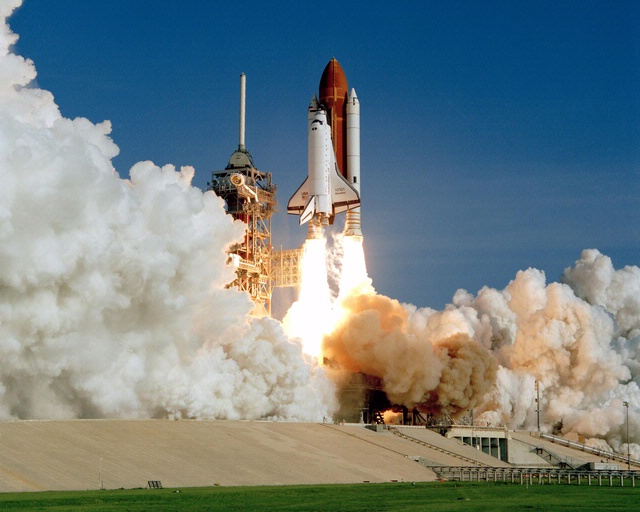
\includegraphics[scale=0.45]{gambar/space-shuttle.jpg}
	\caption{Peluncuran Pesawat Luar Angkasa \emph{Discovery}}
	\label{fig:spaceShuttle}
\end{figure}

Roket luar angkasa merupakan \lipsum[1]
\vspace{0.5ex}

\emph{Discovery} \ref{fig:spaceShuttle} merupakan \lipsum[2]

Beberapa keunggulan dari \lipsum[3][1-2] adalah:
\vspace{0.5ex}

\begin{enumerate}[nolistsep]

  \item Mempermudah \lipsum[1][1-2]
  \vspace{0.5ex}

  \item \lipsum[1][3-4]
  \vspace{0.5ex}

\end{enumerate}
\vspace{0.5ex}

\section{Gravitasi}
\vspace{1ex}

Gravitasi merupakan \lipsum[1]
\vspace{0.5ex}

\subsection{Hukum Newton}
\vspace{1ex}

Newton pernah merumuskan \citep{newtonLaw} bahwa \lipsum[2]
\vspace{0.5ex}

\subsection{Anti Gravitasi}
\vspace{1ex}

Anti gravitasi sendiri merupakan \lipsum[3]
\vspace{0.5ex}